\def\input@path{{../../}}
\makeatother
\documentclass[../../main.tex]{subfiles}

\begin{document}

\section{Понятие о задаче целочисленного программирования}
Итак, давным давно, во время Второй Мировой Войны Европа встала
перед большой проблемой: технологический прогресс 3-ого рейха
породил таких монстров, как самолеты Люфтваффе. Перед правительством
Британии встал большой вопрос по улучшению эффективности ПВО в борьбе
с немецкими самолетами, которые доставляют большие проблемы. Еще с
1935 года Генри Тизерд работал над исследованием эффективности операций
и во время войны его наработки получили большое внимание и развитие. Тогда
был открыт исследовательский центр, где проходила работа по повышению
точности оружия при перехватке самолетов и наведении (как всегда 
война движет прогресс). В центре пытались ответить на вопрос: как из множества
решений выбрать наилучшее? Сначала решения выбирались по наитию, но затем 
появились методы по их расчету и выведению наиболее оптимальных решений (при чем
обоснованных численно). Именно так зародилось исследование операций, основной 
задачей которого является предоставление обоснованных 
данных для принятия решений.

А теперь к теории.

Задача линейного программирования является задачей условной оптимизации, где
следует найти минимум или максимум:
\begin{equation}
    \begin{cases}
        f(x_1, x_2, \dots, x_n) \to min/max \\
        f_i(x_1, x_2, \dots, x_n) \geq b_i, i = 1,2,\dots,n \\
        x_1, x_2, \dots, x_n \in \R
    \end{cases}
\end{equation}

, где $f, f_i$  --- линейные функции.

Подобным образом формулируется задача целочисленного линейного программирования
(все функции $f$ также линейны):
\begin{equation}
    \begin{cases}
        f(x_1, x_2, \dots, x_n) \to min/max \\
        f_i(x_1, x_2, \dots, x_n) \geq b_i, i = 1,2,\dots,n \\
        x_1, x_2, \dots, x_n \in \Z
    \end{cases}
\end{equation}

Вспомним некоторые определения из теории графов.
\begin{defn}
    Неориентированный граф --- это упорядоченная пара $G=(V,E)$, состоящая
    из произвольного непустого конечного множества $V$ и некоторого 
    множества $E$ 
    \emph{неупорядоченных} пар \emph{различных} объектов из $V$.
\end{defn}

Объекты из $V$ --- это вершины.

Объекты из $E$--- это ребра.

Также договоримся, что \emph{неупорядоченные} элементы помещаются в $\{\}$.
Упорядоченные в $()$, что $(b,a) \neq (a,b)$.

Рассмотрим пример и введем еще несколько терминов.
\begin{example}
    Рассмотрим неупорядоченный граф: \\ 
    $V=\{a, b, c, d, e\}$, \\
    $E=\{\{a, b\}, \{b, c\}, \{c, d\}, \{d, a\}, \{c, e\}\}$

    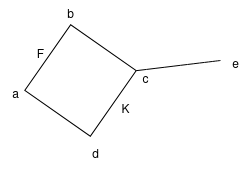
\includegraphics[scale=0.7]{fig1_1.png}
    
    Введем следующие термины:
    $F=\{u, v\} \in E \to u, v$ смежные \\
    $\to u, v$ концевые вершины ребра $F$ \\
    $\to F$ \emph{инцедентно} вершинам $u, v$ \\
    $a, b$ --- смежны \\
    $a, с$ --- не смежны \\
    $a, F$ --- инцидентны \\
    $a, K$ --- не инцидентны \\
\end{example}

\begin{defn}
    Паросочетением в графе $G$ называется подмножество $M\subseteq E$, 
    такое, что в $M$ нету двух ребер с общей концевой вершиной. 
\end{defn}

Например (возвращаясь к рисунку выше) $M=\{\{a, b\}, \{d, c\}, \{c, e\}\}$ 
--- не паросочетание, а $M=\{\{a, b\}, \{c, e\}\}$ --- паросочетание.
\begin{example}[Задача о наибольшем паросочетании]
    Задан $G=(V,E)$, требуется найти паросочетание с максимальным 
    количеством ребер в $G$.

    Заведем переменную для каждого ребра:\\
    $\forall e \in E,$ $x_e = \begin{cases}
        0, $ если ребро $ e $ не входит в подмножество$ \\
        1, $ иначе$
    \end{cases}$

    Количество выбранных ребер: $\sum_{e\in E}x_e \to max$.\\
    
    Далее необходимо ввести ограничения.
    \begin{enumerate}
        \item Пусть $\sigma(v)$ --- множество ребер из $E$ инцедентных 
        вершине $v$ (говоря иначе, ребра выходящие из вершины).
        Первым ограничением будет условие, что инцедентных ребер может
        входить не более \textbf{1} в множество $\sigma$:
        \begin{equation}
            \sum_{e \in \sigma(v)}x_e \le 1, \forall v \in V
        \end{equation}
        \item Также введем ограничение для значений каждой переменной:
        \begin{equation}
            0 \le x_e \le 1, \forall x_e \in \Z, \forall e \in E
        \end{equation}
    \end{enumerate}

    Сумма, обозначающая количество ребер, и введенные ограничения формируют
    целочисленную задачу, допустимым (оптимальным) планом которой 
    может являтся вектор    вида $x=(0, 1, \dots, 1, 1)$.
\end{example}

\begin{example}[Задача о коммивояжоре]

    Дано
    $S=\{1,2,\dots,n\}$ --- количество городов.
    $d_{ij}$ --- расстояние от $i$ до города $j$.

    Коммивояжор выходит из некоторого города, посещает все остальные города
    равно \emph{1} раз и в возвращается в тот город, из которого он вышел.

    Требуется найти маршрут коммивояжора такой, что суммарное расстояние,
    пройденное коммивояжором, минимально.

    
    Для каждой упорядоченной пары различных городов $(i,j)$ введем:
    \begin{equation}
        x_{ij} = \begin{cases}
            1, $ если коммивояжор совершает переход из города $ i $ в $ j \\
            0, $ иначе $
        \end{cases}
    \end{equation}

    Тогда расстояние пройденное коммивояжором будет выглядить:
    \begin{equation}
        \sum_{(i, j)}{d_{ij}x_{ij}} \to min, \\
        1 \le i \le n, \\
        1 \le j \le n, \\
        i \neq j 
    \end{equation}
    
    В результате была записана задача оптимизации, которую необходимо
    минимизировать.

    Далее запишем огреничения и спомагательные уравнения:
    \begin{equation}
        \sum_{j=1}^{n}x_{ij} = 1, i \neq j,
        \forall i \in \{1, 2, \dots, n\}
    \end{equation}
    \begin{equation}
        \sum_{i=1}^{n}x_{ij} = 1, i \neq j,
        \forall j \in \{1, 2,\dots, n\}
    \end{equation}
    \begin{equation}
        0 \le x_{ij} \le 1, x_{ij} \in \Z
        \begin{cases}
            \forall j \in \{1, 2, \dots, n\} \\
            \forall i \in \{1, 2, \dots, n\}
        \end{cases}
    \end{equation}

    Описанные уравнения являются необходимыме условиями для решения
    задачи, но не являются достаточными. Например можно найти такой граф
    (городов), который удовлетворяет условиям 1.6-1.9, но не удовлетворяет
    изначальной задаче (см. рисунок 2). На рисунке города разделены на две
    области, между которыми нету дорог, чтобы коммивояжор мог добраться до
    городов из противоположной области. Например из города $1$ в $k+1$.

    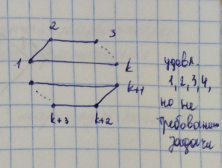
\includegraphics[scale=0.7]{fig2_1.png}

    Для того, чтобы исключить подобные ситуации и сделать задачу решаемой,
    необходимо ввести дополнительное уравнение.
    
    Для каждого города $i \in \{1,2, \dots, n\}$ введем $u_i \in \Z$.

    Для каждой упорядоченной пары различных городов $(i,j)$, где
    $2 \le i \le n$ и $2 \le j \le n, i \neq j$:

    \begin{equation}
        u_i - u_j + nx_{ij} \le n - 1
    \end{equation}

    Выражение 1.10 называется \textbf{ограничение (условие) Таккера}.

    Для решения задачи докажем лемму, убеждающую нас в том, что выражений
    1.6-1.10 достаточно.

    \begin{lemma}
        Ограничениям 1.6-1.10 удовлетворяют все допустимые маршруты коммивояжора
        и только они.
    \end{lemma}
    \begin{proof}
        Покажем, что условия 1.6-1.10 определяют допустимые маршруты
        коммивояжора.

        Достаточно показать, что любой цикл, удовлетворяющий 1.6-1.10
        проходит через город 1.(!!!)

        От противного. Допустим цикл из решения системы 1.6-1.10 не проходит
        через город 1.

        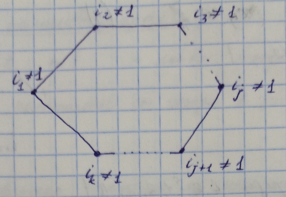
\includegraphics[scale=0.7]{fig3_1.png}
        
        Получим:
        \begin{equation*}
            \begin{cases}
                \forall j \in \{1, \dots, k-1\} \\
                u_{i_j} - u_{i_{j+1}} + nx_{i_ji_{j+1}} \le n-1 \\
                u_{i_k} - u_{i_1} + nx_{i_ki_1} \le n-1
            \end{cases}
        \end{equation*}

        Где $x_{i_ji_{j+1}}=x_{i_ki_1}=1$ так как !TODO!. В этой связи
        получим:

        \begin{equation*}
            n * k \le (n-1)k
        \end{equation*}
        \begin{equation*}
            n \le n - 1
        \end{equation*}

        Получено противоречие. Это значит, что предполагаемого цикла нет и
        любой цикл из 1.6-1.10 проходит через 1. Следовательно цикл всего 1
        --- допустимый маршрут коммивояжора.

        Покажем, что для любого допустимого маршрута коммивояжора, найдутся
        значения переменных, при которых ограничения 1.6-1.10 выполняются.

        Рассмотрим произвольный допустимый маршрут коммивояжора.


    \end{proof}




\end{example}

\end{document}